\documentclass{article}
\usepackage{tikz}

\begin{document}    
    \begin{figure}[h]
        \centering
        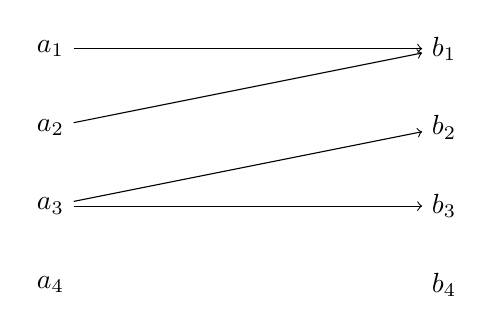
\begin{tikzpicture}
            \node (a1) at (0, 0) {$a_1$};
            \node (a2) at (0, -1cm) {$a_2$};
            \node (a3) at (0, -2cm) {$a_3$};
            \node (a4) at (0, -3cm) {$a_4$};
            
            \node (b1) at (5cm, 0) {$b_1$};
            \node (b2) at (5cm, -1cm) {$b_2$};
            \node (b3) at (5cm, -2cm) {$b_3$};
            \node (b4) at (5cm, -3cm) {$b_4$};

            \draw[->] (a1) to (b1);
            \draw[->] (a2) to (b1);
            \draw[->] (a3) to (b2);
            \draw[->] (a3) to (b3);
        \end{tikzpicture}
        \caption{Not a Function}
    \end{figure}
        
    \begin{figure}[h]
        \centering
        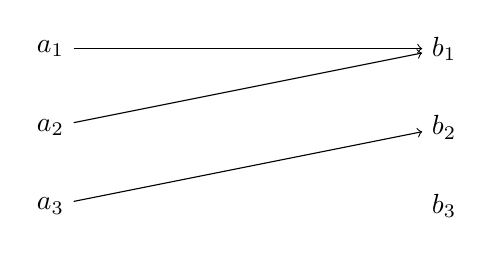
\begin{tikzpicture}
            \node (a1) at (0, 0) {$a_1$};
            \node (a2) at (0, -1cm) {$a_2$};
            \node (a3) at (0, -2cm) {$a_3$};
            
            \node (b1) at (5cm, 0) {$b_1$};
            \node (b2) at (5cm, -1cm) {$b_2$};
            \node (b3) at (5cm, -2cm) {$b_3$};

            \draw[->] (a1) to (b1);
            \draw[->] (a2) to (b1);
            \draw[->] (a3) to (b2);
        \end{tikzpicture}
        \caption{Function}
    \end{figure}

    \begin{figure}[h]
        \centering
        \begin{tikzpicture}
            \node (a1) at (0, 0) {$a_1$};
            \node (a2) at (0, -1cm) {$a_2$};
            \node (a3) at (0, -2cm) {$a_3$};
            
            \node (b1) at (5cm, 0) {$b_1$};
            \node (b2) at (5cm, -1cm) {$b_2$};
            \node (b3) at (5cm, -2cm) {$b_3$};
            \node (b4) at (5cm, -3cm) {$b_4$};

            \draw[->] (a1) to (b1);
            \draw[->] (a2) to (b3);
            \draw[->] (a3) to (b4);
        \end{tikzpicture}
        \caption{1-to-1}
    \end{figure}

    \begin{figure}[h]
        \centering
        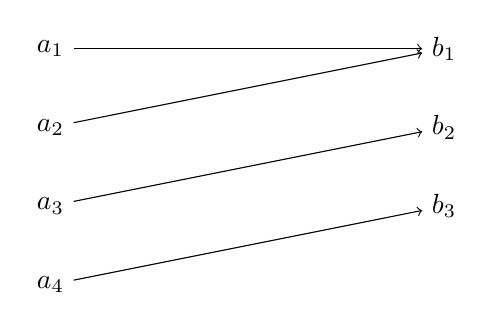
\begin{tikzpicture}
            \node (a1) at (0, 0) {$a_1$};
            \node (a2) at (0, -1cm) {$a_2$};
            \node (a3) at (0, -2cm) {$a_3$};
            \node (a4) at (0, -3cm) {$a_4$};
            
            \node (b1) at (5cm, 0) {$b_1$};
            \node (b2) at (5cm, -1cm) {$b_2$};
            \node (b3) at (5cm, -2cm) {$b_3$};

            \draw[->] (a1) to (b1);
            \draw[->] (a2) to (b1);
            \draw[->] (a3) to (b2);
            \draw[->] (a4) to (b3);
        \end{tikzpicture}
        \caption{Onto}
    \end{figure}

    \begin{figure}[h]
        \centering
        \begin{tikzpicture}
            \node (a1) at (0, 0) {$a_1$};
            \node (a2) at (0, -1cm) {$a_2$};
            \node (a3) at (0, -2cm) {$a_3$};
            
            \node (b1) at (5cm, 0) {$b_1$};
            \node (b2) at (5cm, -1cm) {$b_2$};
            \node (b3) at (5cm, -2cm) {$b_3$};

            \draw[->] (a1) to (b1);
            \draw[->] (a2) to (b2);
            \draw[->] (a3) to (b3);
        \end{tikzpicture}
        \caption{1-to-1 \& Onto}
    \end{figure}
\end{document}
